\documentclass[tikz,border=3pt]{standalone}
\usetikzlibrary{arrows.meta,calc}
\usepackage{amsmath,bm}
\let\boldsymbol\bm
\begin{document}
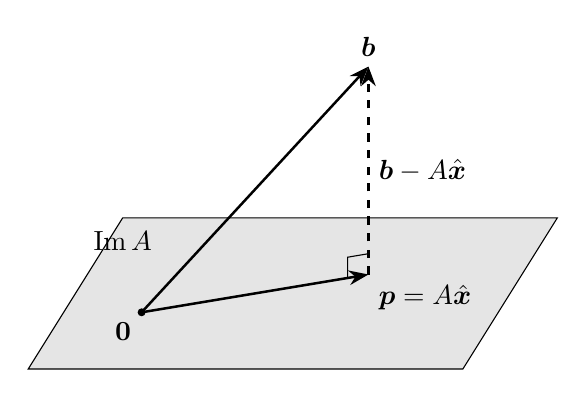
\begin{tikzpicture}[scale=1.2,>=Stealth,line width=0.9pt]
  \fill[black!10] (-1.2,-0.6) -- (3.4,-0.6) -- (4.4,1.0) -- (-0.2,1.0) -- cycle;
  \draw[line width=0.4pt] (-1.2,-0.6) -- (3.4,-0.6) -- (4.4,1.0) -- (-0.2,1.0) -- cycle;
  \node at (-0.2,0.75) {$\mathrm{Im}\,A$};
  \coordinate (O) at (0,0);
  \coordinate (P) at (2.4,0.4);
  \coordinate (B) at (2.4,2.6);
  \draw[->] (O) -- (B) node[above] {$\boldsymbol{b}$};
  \draw[->] (O) -- (P) node[below right] {$\boldsymbol{p}=A\hat{\boldsymbol{x}}$};
  \draw[->,dashed] (P) -- (B) node[midway,right] {$\boldsymbol{b}-A\hat{\boldsymbol{x}}$};
  \draw[line width=0.4pt] ($(P)+(0,0.22)$) -- ++(-0.22,-0.037) -- ++(0,-0.22);
  \fill (O) circle (1.2pt) node[below left] {$\boldsymbol{0}$};
\end{tikzpicture}
\end{document}
